\documentclass[main.tex]{subfiles}
\graphicspath{{./img}}

\begin{document}
    
\section{Proposed system}\label{sec-system}

This section is dedicated to designing the system that will be used to implement ITS in the
vehicle simulator software. A framework dedicated for generic MAS-based ITS system
implementation will be designed, utilizing the principles and paradigms gathered in the
preceding sections (\ref{its}, \ref{mas}). Firstly, the \emph{micro-architecture} will be
defined, i.e. the specification of the system's actors (agents) - their inner structure 
will be defined, as well as interfaces to the environment, and high-level technical specification 
will be proposed - responsibilities of inner components and their inter-relationships.
This will form the elementary foundation that will be used to build an actual system.
The subsequent \emph{macro-architecture} proposal will mainly encompass modes of inter-
agent communication. This outline will form a system specification that will be used 
to build the agent-based ITS framework for IVS software.

\subsection{Agent/micro architecture overview}

As per the previous section(s), where the individual MAS architectures have been reviewed
(section \ref{mas}), it was decided to utilize  the hybrid \emph{\textsubscript{3}T
architecture\footnote{To remind the reader of the architecture's general structure, its
schematic is shown below (fig. \ref{3-arch2}).}} (section \ref{hybrid-arch}), which will offer
sufficient flexibility.  Such modeling flexibility is needed primarily because there won't be a
single, concrete system to model, but rather a generic system that will facilitate arbitrary
agent-based ITS implementation. As such, it makes sense to choose a hybrid architecture, which
will ensure there will be optimal balance between robust, reactive behaviour without giving up
capabilities to model complex behaviour.

Note that the architecture will be formally assume that the its implementation will be realized 
in an Object-Oriented Programming (OOP) paradigm. There are multiple reasons for that. Firstly, 
The nature of agent based systems, having their internal logic and interacting with the surroundings 
through pre-defined interface, corresponds to a large degree to the concepts of OOP, especially
the encapsulation mechanism.

The individual layers/components will be outlined in the following section, in a bottom-up
fashion.

\begin{figure}[htbp]
    \centering
    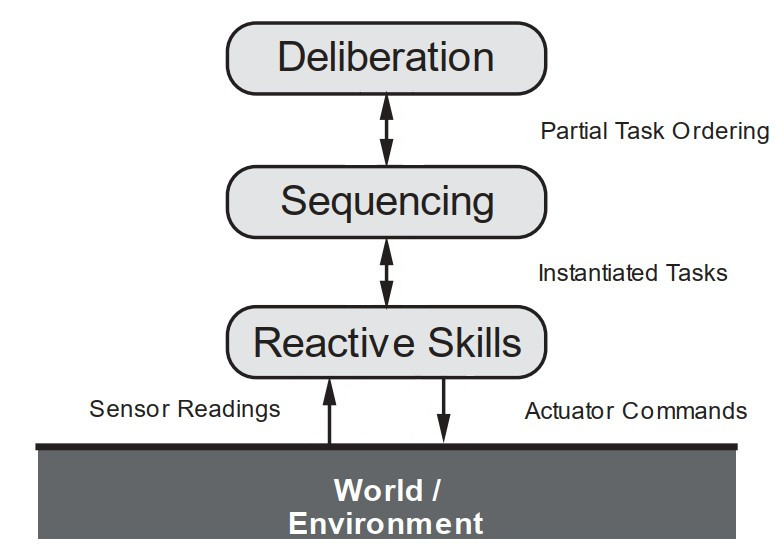
\includegraphics[width=.8\textwidth]{3t-arch.jpg}
    \caption{An architecture model of a \textsubscript{3}T hybrid architecture \cite{Bonasso1995}}
    \label{3-arch2}
\end{figure}

% The elementary characteristics that were defined according to \cite{ParasumannaGokulan2010}
% must shall also be taken into account: 

% \begin{itemize}
%     \item Situatedness
%     \item Autonomy 
%     \item Inferential capability 
%     \item Social behaviour 
% \end{itemize}

\subsubsection{The architecture layers}

In this section, the individual layers of the architecture will be defined. The layers' definition will 
adhere to the characteristics of the \textsubscript{3}T architecture. For each layer, it's purpose and 
relation to other layers will be described, together with technical implementation guidelines, such as 
configuration etc.

\textbf{Reactive skills layer}

This layer encapsulates all the \emph{skills} the agent is able to do. These are the 
most primitive types of its behaviour\footnote{The original author of the architecture refers to them 
as Reactive Action Packages (RAPs) \cite{Firby1987}.}. For example, a skill might be to slow
down or to follow a vehicle in case of vehicle-based agent. Skills can be activated and deactivated based 
on the cognitive capabilities of higher layer (sequencing) and more than one skill can be active at 
any moment, and they should be independent of each other. However, one skill might use output of another 
skill as its input, effectively making a network of skills. By providing skills for elementary operation,
a level of abstraction is created, which emphasizes focus on impacts of task sequencing without being 
overly concerned by how the individual skills interact with the environment. The original article 
proposing the architecture stresses a following canonical approach for skill specification
\cite{Bonasso1995}:

\begin{enumerate}
    \item The skill's input and output specification. Each skill must provide a
description of the inputs it expects and a listing of the outputs that it
generates 
    \item A computational transform This is where the skill does its work. Once a
skill is enabled, it uses this transform to continually recompute its outputs
based on its current inputs.
    \item An initialization routine. Each skill is given the opportunity to initialize itself when the system is started 
    \item An enable function. The sequencer can enable and disable skills Depending on the
    context, a skill is given the opportunity to perform any special start up procedures each
    time it is enabled.
    \item A disable function When a skill is no longer needed, the sequencer will disable it
    and the disable function performs any necessary cleanup actions.
\end{enumerate}

In practice, each skill will be an individual script that will be \emph{asynchronously} run.
Each script will have to implement a \emph{start-up} and \emph{clean-up} function.
Inside the script, it will be possible to interact with the skills inputs and transform them to 
outputs. For instance, mainly will be possible to route output from sensor or communication skills
to other skills that use the outputs. Skills will provide interface to the higher abstraction layer 
through pre-defined events specific to each skill.

In relation to the lower-level skills (i.e. communication and sensory), such skills should be 
able to have configurable physical layer parameters such as signal range or relative service
reliability (error rate). Speaking of error behaviour, a skill should also be able to return a
failure state event to enable fail-safe behaviour. 

\textbf{Sequencing layer}

The sequencing layer is responsible for \emph{execution} of the individual skills, essentially 
controlling which skills to enable/disable to achieve a certain behaviour. It is the 
intermediate layer between the reactive skill layer and deliberative planning layer. 

This layer will feature logic that will be used to accomplish a task in varying circumstances, 
based on the state of the environment or the agent itself. For instance, regarding a driving 
vehicle, a routine task to avoid an obstacle (which is defined by enabling certain skills by
the sequencer) will be handled differently on a road with more than two lanes.

The sequencing layer should not be responsible for more complicated reasoning, but rather 
to define how to handle routine situations. The responsibility for high level planning to achieve 
a global goal for an agent is reserved for the upper (deliberation) layer. The sequencing layer's 
role in relation to the upper layer is to provide an additional layer of abstraction.

To formalize the purpose of this layer in the proposed system, it should contain definitions 
of which skills to enable to complete a rudimentary task, managing sequences of common skills
along with logic that will account for completing them in different scenarios. The layer
interact with both the lower (skill) layer - interacting through events triggered by individual
skills to alter skill execution, and the upper (deliberation) layer. 

% There will be \emph{two} separate queues, one for basic skill queuing and the second priority queue that 
% will be used when agent behaviour needs to be temporarily altered. each inducing slightly different effect on currently executing 
% skill. The second queue type will :

% \begin{itemize}
%     \item \textbf{Basic queue} - The default queue with no special effect on current executing skill. After the current 
%     skill finishes, the next skill in the queue gets initiated and executed.
%     \item \textbf{Priority queue} - When skills are added to this queue, the currently executing skill gets immediately 
%     suspended and the newly added skills get executed instead. When this higher-priority queue is cleared, the 
%     previously suspended task will continue to execute.
% \end{itemize}

% Because indirect communication (i.e. 
% broadcasting) will be featured in the proposed system, asynchronous skill sequencing will also be 
% implemented using \emph{callbacks}. Usage of this feature can be simply argued by the fact that in traffic, 
% the state of environment is changing rapidly, thus relying on sensory feedback would often not be enough 
% to avoid faulty behaviour. Furthermore, there is a vast number of ITS solutions that utilize the 
% broadcaster-subscriber principle, such as CACC systems and C-ITS systems in general.

\textbf{Deliberation layer}

The deliberation layer (also referred to as the planner) synthesizes high-level goals into a
partially ordered \emph{plan}, listing tasks that the agent has to perform, in order to achieve
the specified goal. Ultimately, the main purpose of the layer is to manage tasks execution to
achieve a specified goal. For example,  More generally, a goal could be something that the user
wants the agent to accomplish, for example, a vehicle's goal is to arrive to its final
destination.

Thanks to the abstractions provided by the two lower layers, the planner can be represented as
a conditional state-based model, vastly simplifying its definition \cite{Bonasso1995}. In
addition to this, it will be possible to add parameters to goal definition. The final version of the plan 
will then be generated based on parameter values and internal logic that will process them.

In practice, the most trivial specification of the deliberation layer will consist of:

\begin{enumerate}[label=\alph*)]
    \item \textbf{Primary goal} - The main objective that the agent was designed to perform.
    \item \textbf{Fail-safe goal} - The desired outcome of agent's behaviour in case an unexpected 
    failure occurs in any its components or when the agent fails to achieve the primary goal. 
    For example performing a Minimum Risk Maneuvre in vehicle based agents
    \cite{WorkingAutonomous2022}. %should I cite this???
 \end{enumerate}

For more complex behaviour, additional goals can be specified. In that case, the choice which 
plan to prioritize will be determined by sets of pre-conditions and constraints represented by
the agent state.

To sum it up, a detailed view on the individual components of the architecture and their
interface is on the figure (\ref{arch-proposal}) below.

\begin{figure}[htbp]
    \centering
    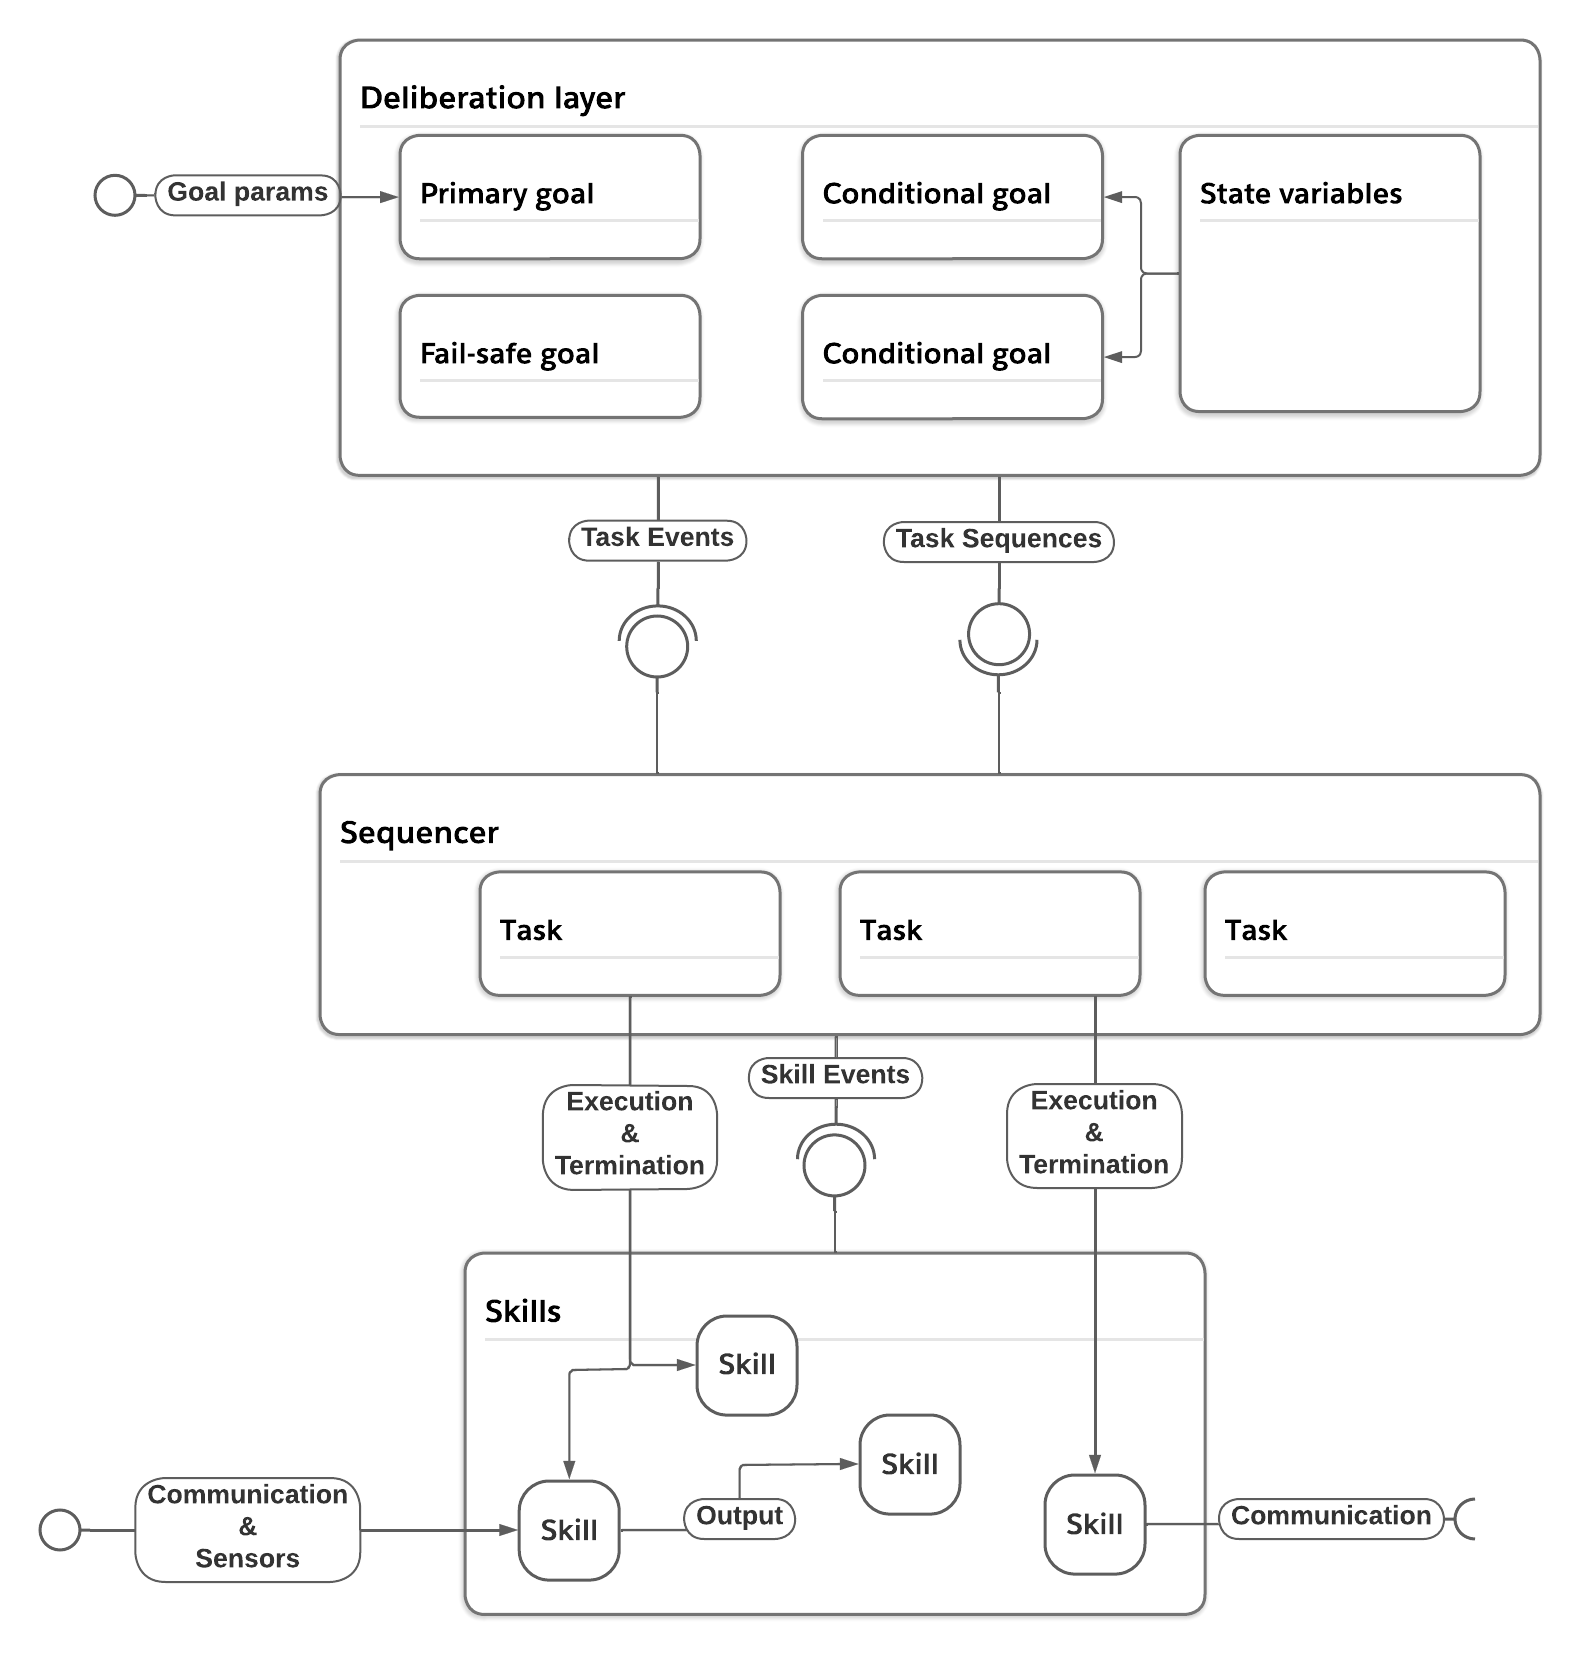
\includegraphics[width=\textwidth]{architecture-proposal.png}
    \caption{An overview of the proposed 3T architecture}
    \label{arch-proposal}
\end{figure}

% The most trivial option will be to create \emph{static} workflows, which will work under the
% assumption that workflow will not get interrupted or reach a fail state at any point, i.e. is
% expected to finish. The second option will be to create \emph{dynamic} workflows, which will enable
% re-planning according to changing environment conditions.  Re-planning will occur when it's
% triggered by one of the \emph{exit state} of agent's skills. The triggers will happen under the
% following conditions: skill returning a \emph{failure state}, callback triggered by one of the 
% \emph{physical modules} (e.g. messages from other agents or sensory input).
% This will cause the planner to re-plan by adding appropriate steps to the executing workflow to
% optimally adapt to the situation. Therefore, the framework will offer to define conditions
% under which additional steps will get added to ideally achieve a \emph{fail-safe behaviour}.
% For better logical organization, the added steps (which are identified to most often execute in
% a certain sequence) could be grouped into \emph{subtasks}.

% To further improve the resilience of the
% system, the executing workflow can be configured to reach a \emph{workflow failure state},
% which will trigger a pre-determined fail-safe workflow, that is composed of entirely different
% steps, essentially throwing away the previous, failed workflow.  This will be useful when the
% planner will run out of options to adapt to the situation, settling for a goal that would
% destabilize the system as least as possible. For example, autonomous vehicles performing a
% \emph{minimum risk maneuvre} to come to a standstill on the road side when the expected driver
% input is not received \cite{WorkingAutonomous2022}.

\pagebreak
%%%%%% I'd move this further down to the full implementation phase
% Firstly, the matter of how much logic has to be pre-defined in the framework and how much will be left to the implementation 
% itself needs to be discussed thoroughly in this case, as there is a non-trivial task. The



\subsection{Macro architecture}

\subsubsection{Communication protocol}

As has been discussed in the previous sections, communication plays an important part in 
MAS, mainly because it vastly extends capabilities of interaction between agents and thus 
the ability to model more complex behaviour. In section (\ref{sec-acl}), the ACL communication 
standard for MAS has been introduced and requirements for the protocol implementation have 
been presented. To be able to 
utilize the communication, requirements for messaging utility and high-level implementation 
details will be presented. 

\subsubsection{Broadcasting}

The first type of communicating that will be implemented is message broadcasting. This is 
argued by the fact that ITS uses information broadcasting in a lot of cases.
Generally, there are mostly two types of service messaging in ITS \cite{Santa2013}:

\begin{itemize}
    \item \textbf{Periodic status exchange} - ITS services often need to know about 
    status of other actors, such as terminals or vehicles. These periodic updates 
    often include basic status messages such as location, ID, speed, etc.
    \item \textbf{Asynchronous notifications} - Messages that are used to inform 
    about specific event, usually related to a specific service and functionality.
\end{itemize}

%  Especially the C-ITS platform, which uses two types of (middleware) messages,
% specified by the European Telecommunication Standards Institute (ETSI):

% \begin{itemize}
%     \item \textbf{Cooperative Awareness Message (CAM)} which are "heartbeat" periodically 
%     broadcasted messages
%     \item \textbf{Decentralized Environmental Notification Message (DENM)} which are event-
%     triggered messages broadcasted to alert road users.
% \end{itemize}

The framework should therefore support message broadcasting for both synchronous and 
asynchronous events, which should ensure that all potential use-cases are covered. 

\subsubsection{Implementation}

As has been mentioned above, the ability to broadcast and subscribe to said broadcast should be
handled by a separate skill component. Upon skill initialization, the communication skill will
connect to a communication channel and listen or send messages. Each communication stream will have 
to specify what kind (group) of messages it will be sent through it, so that agents can be set up to 
only use channels with messages relevant to them. The agents will be able to react to received
messages by sending an internal event message to the sequencer. 

Given the great utility of C-ITS system and identified similar characteristics and use-cases 
with agent-based systems (discussed in section \ref{sec-research}), the framework will feature 
V2V communication support with standardized message structure and semantics out-of-the-box; 
Namely the Cooperative Awareness Message (CAM) and Decentralized Environmental Notification Message (DENM).

\subsubsection{ETSI message services}

Due to wide range of beneficial use-cases for the aforementioned types information sharing
types (periodic status exchange \& asynchronous notifications), ETSI has defined two basic
messaging services; The CAM message (synchronous status update) and the DENM message
(asynchronous notifications). Both message types will be described along with the implementation 
details.

\textbf{Cooperative Awareness Message}\smallskip\newline

The CAM message is specified by the Cooperative Awareness Basic Service. By definition, CAM
provides by means of periodic sending of status data a cooperative awareness to neighbouring
nodes. From the message propagation point of view, the CAM differs from the DENM message by 
only allowing \emph{single-hop transmission}. This way, only vehicle sin the relative vicinity 
of the broadcasting vehicle will receive the message. CAM messages should be then processed by 
the CAM Management component to apply additional logic \cite{ETSI2014}. For example the CAM Management can 
detect a Slow Vehicle Warning from analyzing received CAM mesages from a particular vehicle. 
In other words, the receiver is expected to evaluate relevance of the contained information.
The CAM service has its message format specification, which is found on figure (\ref{cam-spec}) below. 

\begin{figure}[htbp]
    \centering
    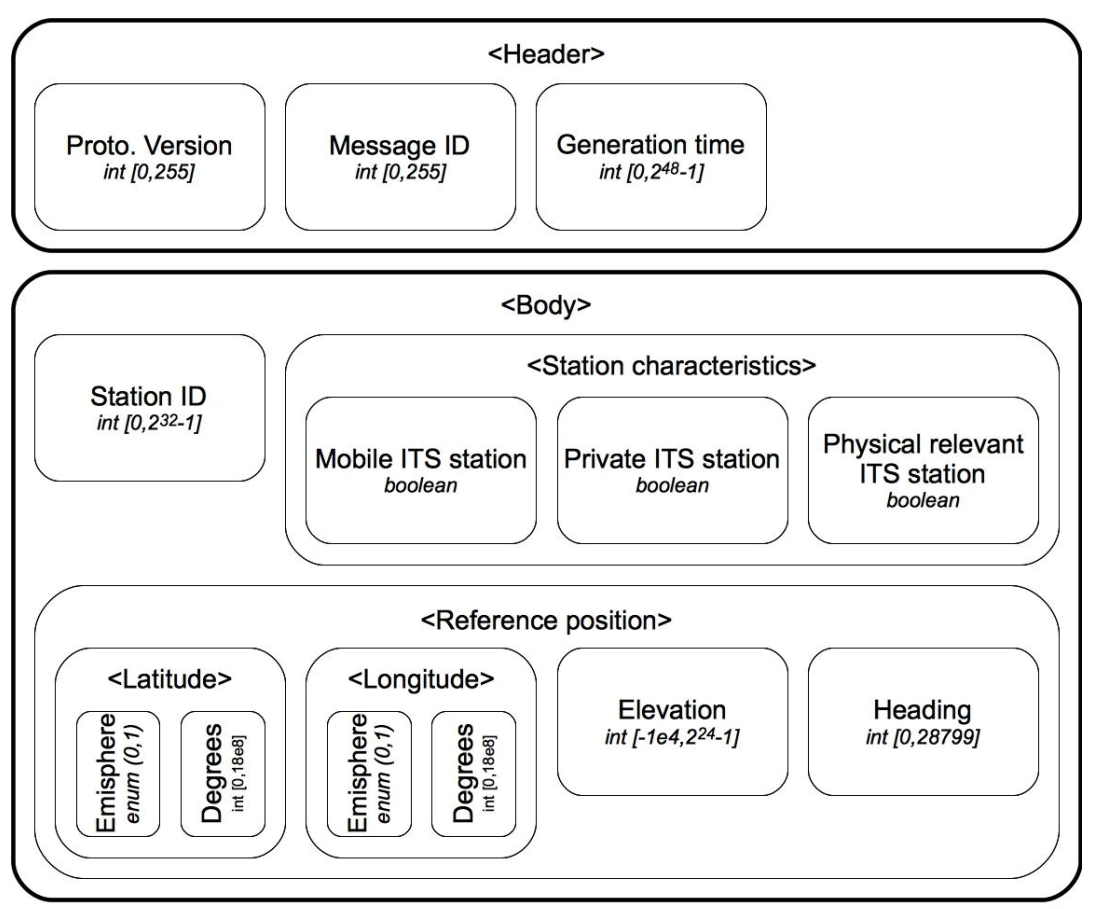
\includegraphics[width=.9\textwidth]{cam-spec.png} 
    \caption{The CAM message specification \cite{Santa2013}}
    \label{cam-spec}
\end{figure}

\textbf{Decentralized Environmental Notification Message}\smallskip\newline
Instead of vehicle/station status update, DENM messages directly carry traffic safety-related 
information, characterized by \emph{event type} identifier. Another difference from the previous 
message type is that DENM messages are \emph{multi-hop}, and their range is expressed by geo-validity 
specification. Among other attributes, the DENM message contains attributes for message generation 
frequency or temporal validity threshold (expiration time). Despite specifying such 
attributes, it is still up to the receiving station/vehicle to determine information relevance
\cite{ETSI2019} and whether to take further actions like displaying the message to the driver.
The DENM service message specification is on the figure (\ref{denm-spec}) below.

\begin{figure}[htbp]
    \centering
    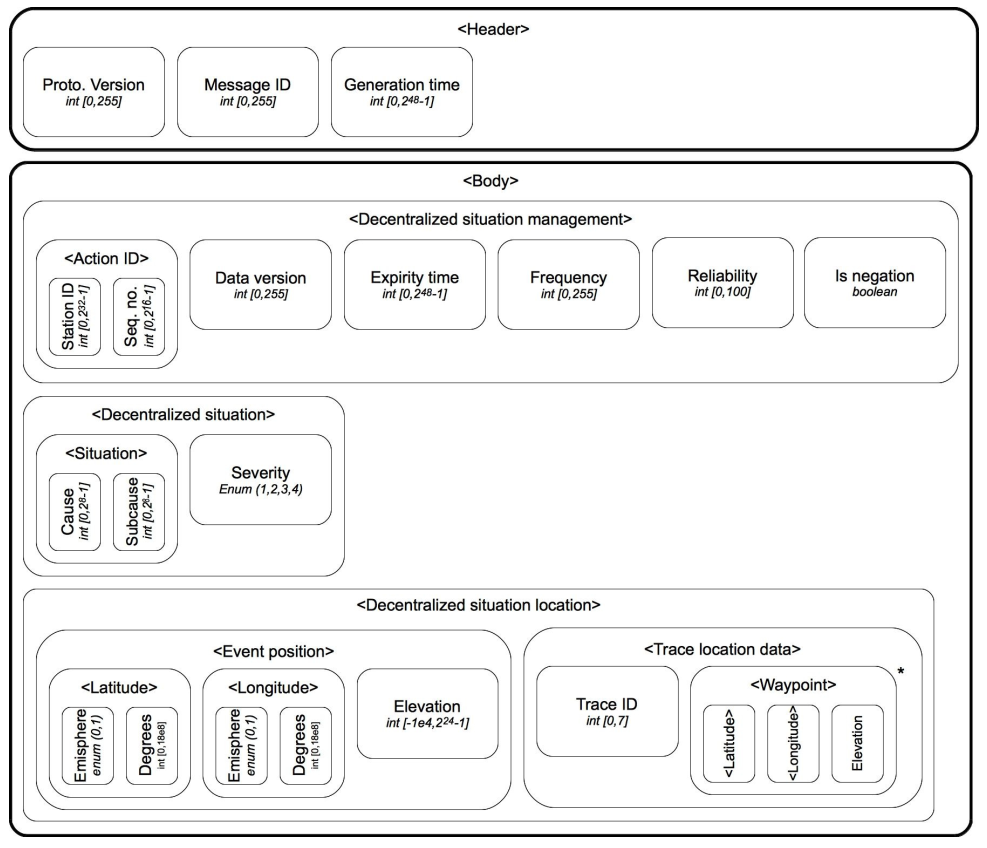
\includegraphics[width=.9\textwidth]{denm-spec.png}
    \caption{The DENM message specification \cite{Santa2013}}
    \label{denm-spec}
\end{figure}

\subsubsection{Negotiation \& Agreement}
\fbox{\begin{minipage}{\dimexpr\textwidth-1em}\textbf{\large I am still not sure if I should
include the following sections related to conflict resolution as I don't know if pursuing this
complex topic would bring substantial value to the proposed system}\end{minipage}}

% still quite too theoretical, not related to actual implementation. not sure if it should be here
Negotiation between agents is important especially when wo agents run into each other, 
followed by the currently executing skills of the agents getting interrupted. In other words, 
The best course of action of one agent is not necessarily best to the other. This is more than
likely to happen in environments where multiple agents share the same resource and their state
is defined on the same domain, which is often the case. As such, the theory of games is formally 
used to model these interactions \cite{Binder2022}. 

This is quite different from the principles of agent cooperation. In cooperation negotiations, 
the worst-case scenario improvement as opposed to working individually is net-zero. \cite{Binder2022}
defines four speech acts in agent negotiation, as seen on fig. (\ref{fig-speech-acts}). This is 
inherently contrary to the statement made in chapter (\ref{mas-interaction}), where it was suggested 
that agent cooperation should be emphasized. As agents are formally modelled as self-interested, 
it cannot be guaranteed that they won't encounter conflicts between each other. Therefore, modelling 
cooperation before figuring conflict resolution would inherently result in a more fragile system 
more prone to malfunction. 

\begin{figure}[htbp]
    \centering
    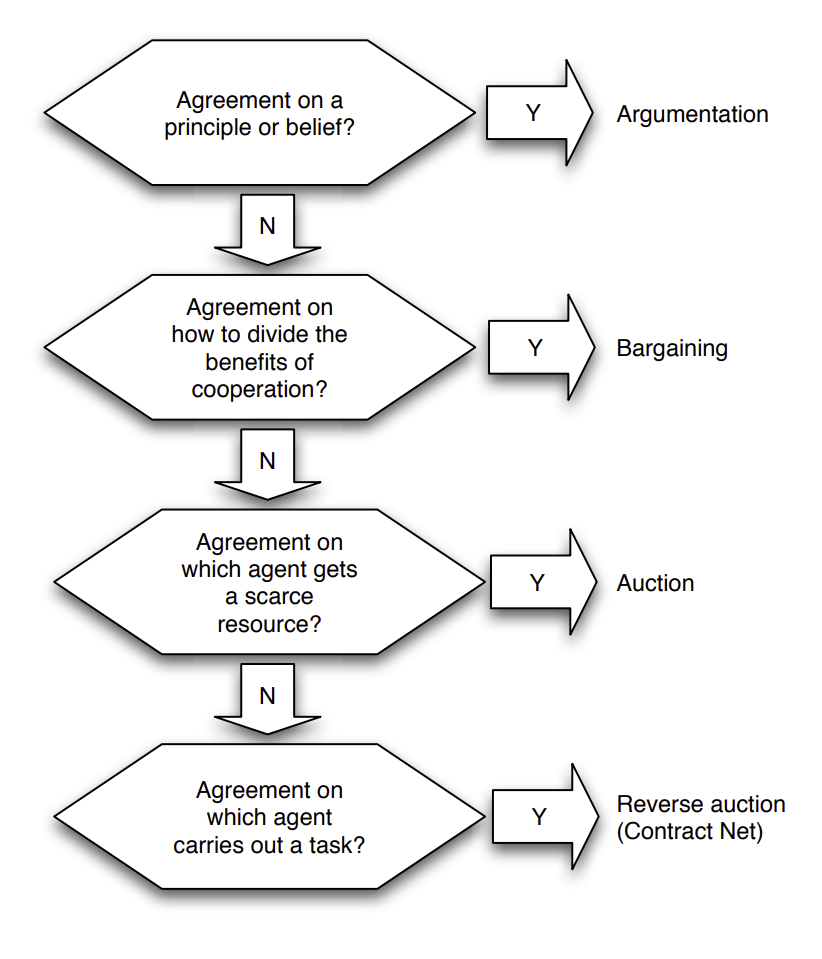
\includegraphics[width=.8\textwidth]{speech-acts.png}
    \caption{Types of agent negotiation \cite{Binder2022}}
    \label{fig-speech-acts}
\end{figure}

\subsubsection{Conflict detection}

As has been argued above, because of scope limitation of this thesis, 
conflict resolution as a system functionality should precede cooperation. The cooperation 
abilities of agents can be added later by extending the framework.
This decision will theoretically lead to better system stability, before offering extended
behaviour possibilities. 

The first step is to have a way for agent to determine a conflict has happened. Agents wouldn't be 
able to resolve conflicts if they didn't know it has occurred. To comply with the \textsubscript{3}T
architecture topology defined above, this should be handled on the reactive skills layer. 
Consequentially, detected conflict will be handled through a dedicated skill module. If an
agent is expected to run into a conflict with another agent (of the same 
 type), if will have
to be equipped with a dedicated skill that will behave as a sensor detecting conflict 
with the implementation left to specific use-case. In other words, the logic for conflict detection will be 
left to define together will specific agent and its properties, and other modules.

It needs to be said that when one agent detects a conflict through one of its modules, it will 
be required to inform other agents about the conflict so that all involved agents will be
aware of the situation. 

%add an image? 

\subsubsection{Conflict resolution}

Now that the conflict detection process was defined, in that case, it will be possible to build
on it to define how conflicts will be resolved. Considering the findings in chapter
\ref{sec-conflicts}, the simplest tool to resolve conflicts is to define hierarchy in the
agent. In order to avoid more complex mathematical reasoning models \cite{Binder2022},
hierarchy, along with agent-bound state variables can be used as a bidding resource. Whichever
agents is able to bid the highest value will get priority in conflict resolution (e.g. by being
able to act in its own interests).

To facilitate the communication related to conflict resolution \& bidding, the FIPA message
standard will be used.  The FIPA standard offers pre-defined messages for such situations -
most importantly the \texttt{Call For Proposal (CFP)} and \texttt{Propose} messages. Although
it was mentioned that agents are self-interested, in order to make things simpler, agents will
assume that the counterparty in conflict is truthful and only bids resources that are
available to them. Also, deciding which bid proposal has won will be handled by the agent that
had called for the proposal, so the counterparty will assume that the deciding agent is
truthful and decided correctly according to the bids. 

% \textbf{Example}

% To illustrate how the system would work in practice a sample scenario is presented below on
% figure (\ref{agentReplanning}), where the agents are drivers/vehicles. The scenario demonstrates 
% how agents achieve their goals using the three layers, as well as conflict detection and resolution.

% There are two vehicle agents (\texttt{A}, \texttt{B}) in the scenario, which both have three skills defined:
% \texttt{drive}, \texttt{avoid:object} and \texttt{wait} and \texttt{negotiate}. Both vehicle
% agents have a goal not to crash and keep a certain speed. To ensure a fail-safe behaviour, a
% dynamic workflow is used, defined as a mapping
% (\texttt{failed\_skill}$\rightarrow$\texttt{safe\_skill}): 

% \begin{itemize}
%     \itemspacing{.5}
%     \item \texttt{drive} $\rightarrow$ \texttt{avoid:object}
%     \item \texttt{avoid:object} $\rightarrow$ \texttt{wait}
%     \item \texttt{wait} $\rightarrow$ \texttt{fail\_goal} (after a timeout for example)
% \end{itemize}

% The mapping of the \texttt{negotiate} skill is \texttt{drive} or \texttt{wait} based on 
% a negotiation result for each involved agent.

% \begin{enumerate}
%     \item Both agents do not detect any obstacles in their surroundings, so the planner
%     initializes a plan with only the \texttt{drive} skill sequenced, which gets executed. 

%     \item Agent (\texttt{A}) spots an obstacle in his way (an oil spill). This makes the
%     \texttt{drive} skill fail and (\texttt{A})'s planner has to re-plan to reach its goal (not
%     crash). The failed skill's fail-safe skills are retrieved (\texttt{avoid:object})
%     and added to the new plan. The new plan is initialized with the two
%     following skills sequenced: \texttt{avoid:oil\_spill} $\rightarrow$ \texttt{drive}.
    
%     \item However, this plan also fail, as agent (\texttt{B}) detects a path conflict, consequentially 
%     informing agent (\texttt{A}) about it. They now have to negotiate to reach an agreement and
%     resolve the conflict using auction-like bidding. The agent (\texttt{B}) wins the bid, due
%     to being in a right lane and so agent (\texttt{A}) is forced to give way. The planner
%     creates a new plan: \texttt{wait} $\rightarrow$ \texttt{avoid:oil\_spill} $\rightarrow$
%     \texttt{drive}.
    
%     \item The individual skills finish successfully and the agents' goal is fulfilled.
% \end{enumerate}

% \begin{figure}[htbp]
%     \centering
%     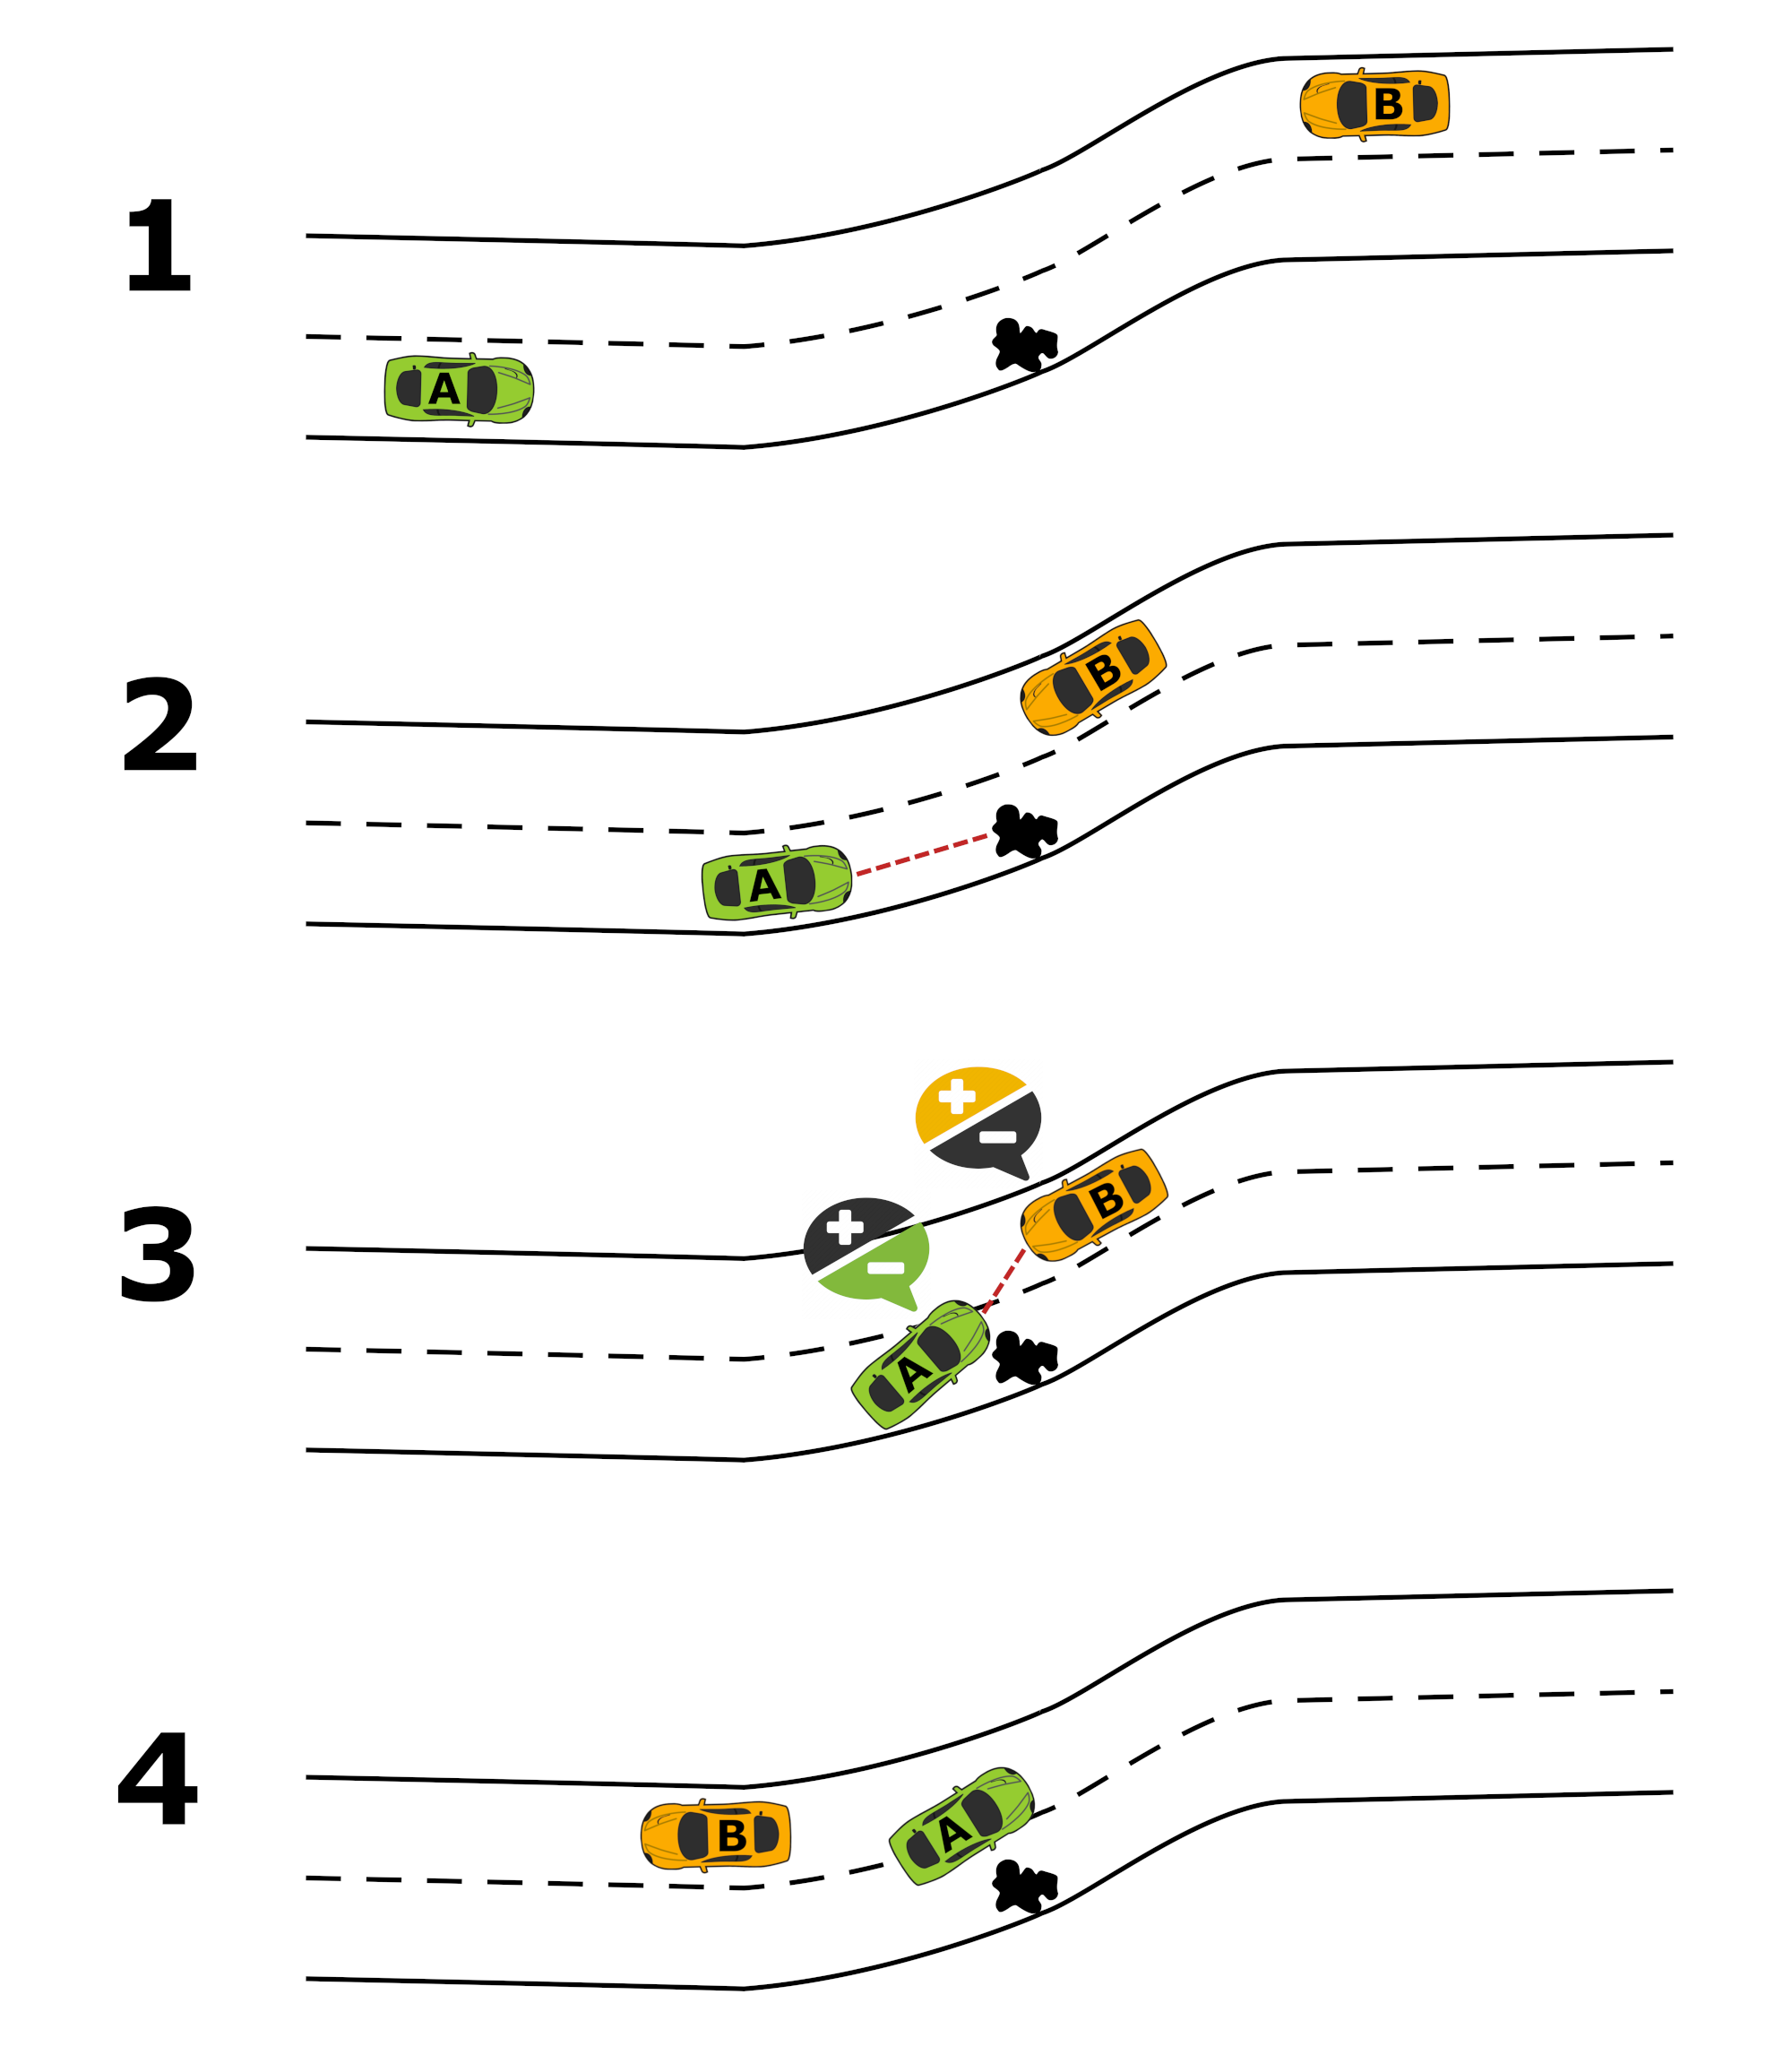
\includegraphics[width=.8\textwidth]{AgentPlanning.png}
%     \caption{An example behaviour of vehicle-based agents using the proposed architecture}
%     \label{agentReplanning}
% \end{figure}

\subsection{System requirements}

To sum up the topic discussed in previous chapters, requirements for framework implementation
are presented in the table (\ref{sys-requirements}) below. This will ensure that when
integrating this ITS framework into existing system (i.e. IVS software), the requirements will
be organized and kept as a reference, helping achieve the desired functionality. Especially
when later choosing a library/framework to help build the framework. 

\begin{table}[htbp]
    \small
    \caption{Proposed system requirements}
    \centering\begin{tabular}{>{\footnotesize}p{.9\textwidth}}
        \toprule 
\emph{\textbf{A}\quad MICRO-ARCHITECTURE REQUIREMENTS}\\ \midrule
\textbf{Requirement 1}: The framework should be a multi-agent based system, supporting more actors 
that are able to act independently, having their own logic and able to make decisions based on their 
own perception of the environment.
\\ \midrule
\textbf{Requirement 2}: The framework will be based on the \textsubscript{3}T architecture. 
This primarily means implementation of the three layers of logic that offer complex behaviour 
modelling.
\\ \midrule
\textbf{Requirement 3}: The framework's architecture should be modular enough to support broad 
spectrum of ITS implementation.
\\ \midrule
\textbf{Requirement 4}: The implementation of a particular ITS-agent's elementary
capability should be done using elementary skill modules. The skill modules must provide a
pre-defined input and output interface.
\\ \midrule
\textbf{Requirement 5}: The executing skills should be able to run asynchronously/concurrently to improve 
performance. The Sequencing layer must be able to manage the asynchronous workflow to avoid errors.
 \\ \midrule
\textbf{Requirement 6}: Interaction between the three layers will be done using events. The 
receiving layer must be able to act upon the received event appropriately based on event type.
 \\ \midrule
\textbf{Requirement 7}: Sensory and communication capability of an agent will be incorporated 
as a separate skill module.
\\ \midrule
\textbf{Requirement 8}: The sequencing layer should ensure that tasks should complete successfully 
in most expected conditions. Failure to execute a task must be reported to the upper layer using an 
appropriate event.
\\ \midrule
\textbf{Requirement 9}: At minimum, an agent should have \emph{two} goals defined - the main goal
and a backup, fail-safe goal that will act as a safeguard when agent is not able to achieve the main 
goal. \\ \midrule
\textbf{Requirement 10}: It should be possible to parametrize the desired goals in order to provide 
more details about the desired behaviour of the agent.
\\ \midrule 
\textbf{Requirement 11}: It should be possible for an agent to adapt to the environment by dynamic re-planning.
Re-planning will initialize a new plan with adapted specification of tasks.
\\ \midrule
\emph{\textbf{B}\quad MACRO-ARCHITECTURE REQUIREMENTS} \\ \midrule
\textbf{Requirement 1}: Agent should be able to communicate with others through a dedicated communication 
interface, with pre-defined semantics. The communication should also adhere to the ACL-compliance requirements 
mentioned in section \ref{sec-acl}.
\\ \midrule
\textbf{Requirement 2}: The supported communication modes will be both direct (messaging specific agents) and indirect  
(broadcast \& subscription). 
\\ \midrule
\textbf{Requirement 3}: The framework will support the CAM and DENM message standards out-of-the-box.
\\ \midrule
\textbf{Requirement 4}: Agents equipped with communication skill module should be able to act upon received information
by triggering an appropriate event to the sequencer. 
\\ \midrule
\textbf{Requirement 5}: Where applicable, agents should be able to detect conflicting intentions with other agents
while executing their tasks. The conflict detection will be implemented as a module on the reactive layer.
\\ \midrule
\textbf{Requirement 6}: On conflict-detecting agents, they must come with a communication module, to be able to 
notify other about the conflict or receive such notification. 
\\ \midrule
\textbf{Requirement 8}: Conflict resolution should be done by bidding a pre-defined resource(s). Hierarchy level can 
also count as a resource.
\\ \bottomrule
    \end{tabular}
    \label{sys-requirements}
\end{table}
\clearpage

\subsection{Conclusion}

In the preceding sections, the multi-agent system framework was proposed. This framework will be used to implement various 
suitable ITSs into an interactive vehicle simulator. The system was described both on micro and macro level. The micro level 
mainly addressed specification of inner architecture of individual agents, how they will achieve their goals using their 
own intelligence. For building independent agents that need to be flexible in terms of their capabilities, the \textsubscript{3}T
architecture was chosen and the individual layers of the architecture were specified in detail, specifying their responsibilities
and capabilities. 

Afterwards, the macro architecture was specified, addressing mainly the ways of how agents will interact with each other. 
Firstly, the communication interface was defined, including how agents will be able to use it on micro-architecture level.
Building upon that, the ways of how conflicts between agents are handled was proposed, utilizing communication to resolve 
conflicts through resource bidding. 

With the micro- and macro-architecture being specified, the final requirements for the system implementation were proposed, 
which aim to help ensure that the software framework will be able to facilitate ITS implementation into IVS software in an 
organized way, with a high system resilience.

\section{System implementation}

With the finished system specification, it should be discussed which tools should be used to build the software framework. 
First off, it is important to analyze the IVS simulation system/software (i.e. the super-system) that
the proposed framework will be incorporated into. An effort should be made to maximize the super-system acceptance of 
this system by choosing an optimal tool-set for its implementation. This, for the most part,
refers to an optimal choice a programming language and a subsequent agent-based modelling
library to use (if there will be any), also due to this being one of the primary tasks of this thesis. 
Therefore, the next section will be devoted to introduction to the IVS software.

\subsection{Simulator software}

The particular simulator software that is being used at the university's faculty is being
developed using the \emph{Unity} game engine, developed by Unity Technologies. The game engine
was first released in 2005 and has been used to develop numerous simulators as well as other
video games ever since \cite{UnityTechnologies2022}.  Unity has also been used as a tool in
physical product modelling, AI \& machine learning and digital twins, used in many industries
\cite{UnityTechnologies2022a}.  The main strengths of Unity are multi-platform development
support, virtual reality development support, good community support (including its own asset
store) and good documentation. The game engine has got its own development environment, which 
can be seen on figure (\ref{unity}) below.

The game engine's runtime is written in the C++ programming language, but the scripting API 
that it offers is in the C\# language. Consequently, the libraries that will be used to develop 
the system should ideally also be .NET based to achieve maximum customization and interoperability.
Potentially, the Unity's Asset store could offer MAS packages, directly utilizing Unity's API.

\begin{figure}[htbp]
    \centering
    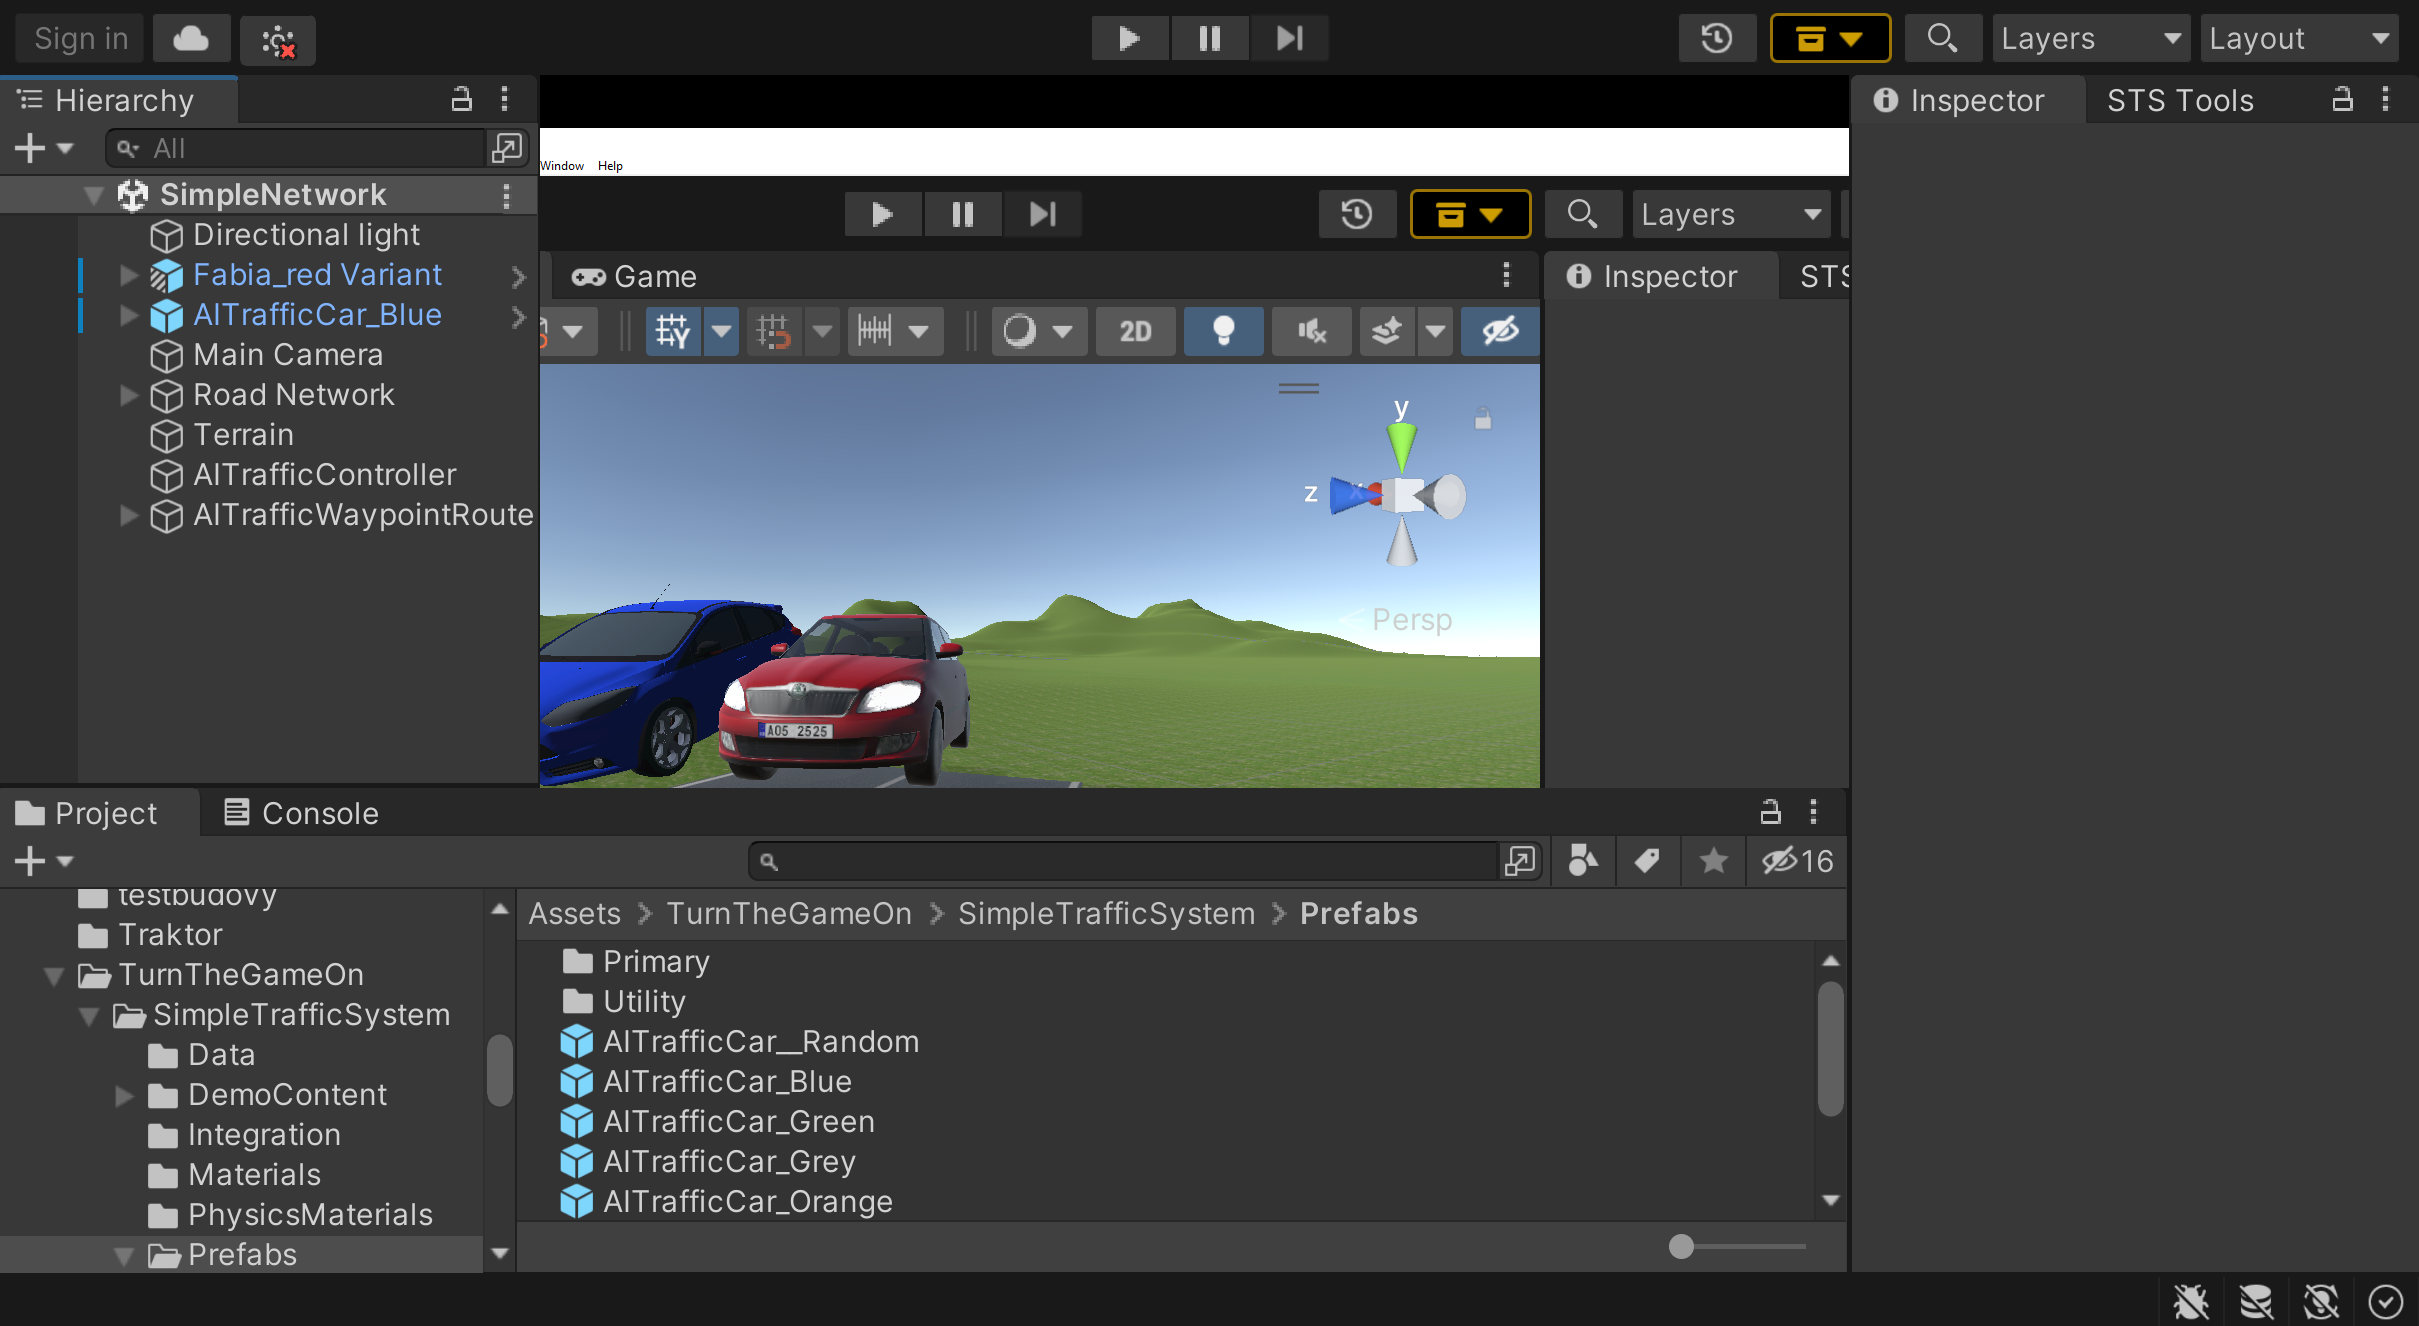
\includegraphics[width=.9\textwidth]{unityUI.png}
    \caption{The Unity development platform UI}
    \label{unity}
\end{figure}

\end{document}
